% Description of your design
\section{Design}
\label{Design}
While every effort was made to meticulously plan out the program structure prior to assigning tasks within the team and beginning to produce source code, inevitably some elements of the program design were altered on an ongoing basis. The team initially envisaged the program being laid out in much larger sized objects than in the final project; for example we would initially have expected to include the input functionality in one class wheras in reality five classes were involved in initiating the program before any computation was done. 

Much of these alterations from the initial idea of the program were guided by the \textit{Single Responsibility Principle} of object-orientated programming that says that each class should perform only one specific function. The team endeavoured to follow this principle where possible which led to the addition of many classes; where once we had a single class for program input we finished with seperate classes to read in data provided as arguments by a user, to extract data from a configuration file provided by the user via the arguments, and to read a bitmask ASCII file.
\begin{figure}
   \begin{center}
      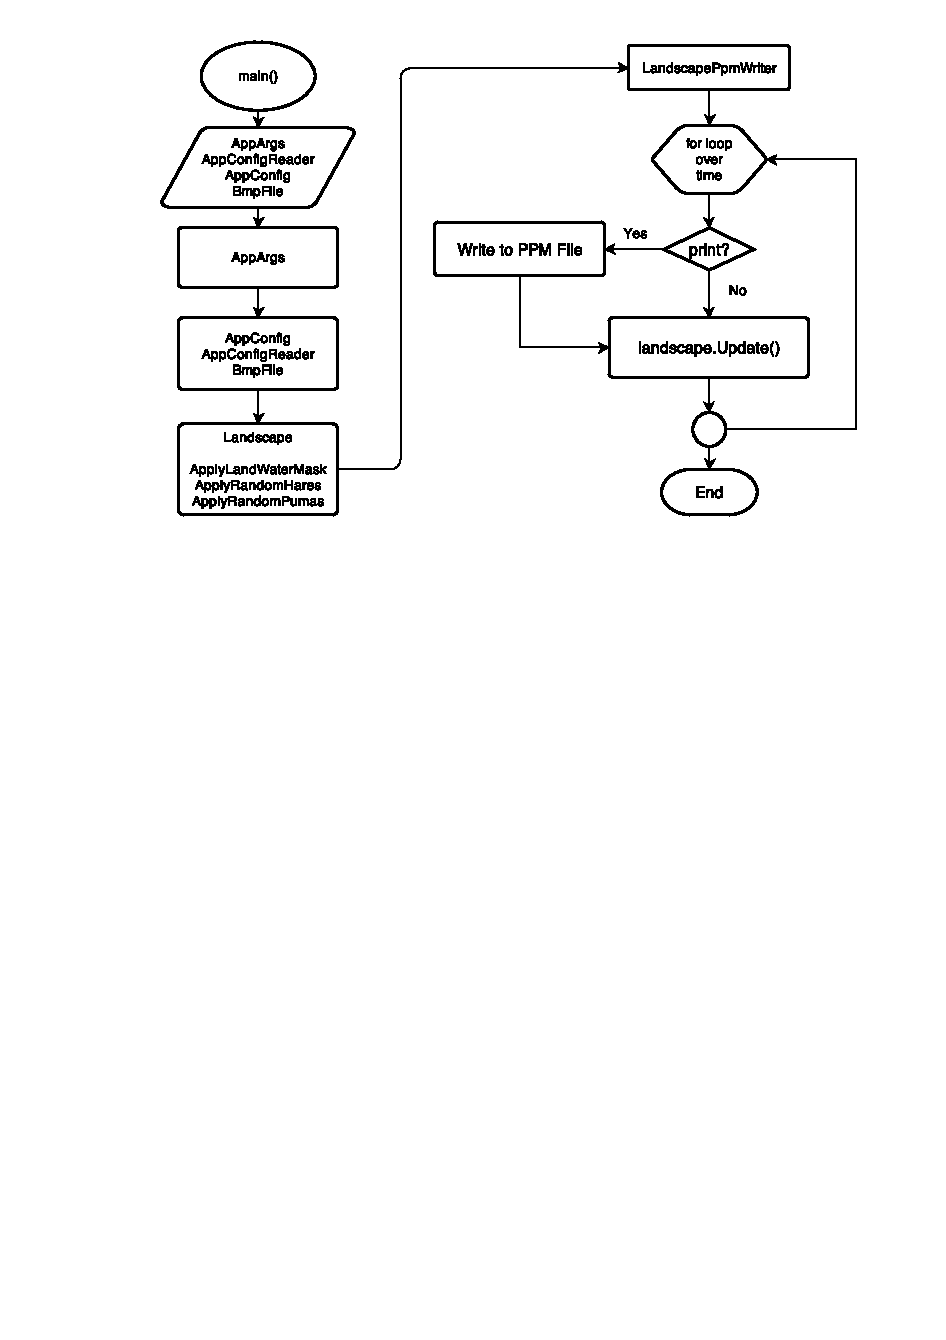
\includegraphics[width=\textwidth]{PS-Coursework-Flow.pdf}
   \end{center}
   \caption{Flow chart representation of the team's program }
   \label{fig:DesignFlowChart}
\end{figure}

Despite our program modules becoming more specialized over the course of implementation the flow generally remained the same. First, the user is to be able to provide the \textit{land/water mask} file that defines the land available to the simulation, as well as a configuration file in which they will pass the desired landscape dimensions\footnote{The dimension passed via the configuration file can be different to that of the passed \textit{land/water mask}, the program will work with the overlap of the two}. This is all done with a combination of \texttt{AppArgs}, \texttt{AppConfigReader}, \texttt{AppConfig}, and \texttt{BmpFile} classes.  

Next, this information is fed into the \texttt{Landscape} class which allocates and initializes the array to hold the population data as well as the details of the land; it can apply a random distribution of Hares (via the \texttt{ApplyRandomHares} function) or Pumas (via \texttt{ApplyRandomPumas}) to the Landscape array, or apply distributions as defined by an array type PopulationMap (via the \texttt{ApplyPopulation} function)\footnote{PopulationMap is a array type defined from the Array2D template in the Landscape class header.}. The latter function was used in performance testing.

As well as performing the last of the initialisation of the program, the Landscape class also contains the main compoutational engine of the program; it implements the discrete relations provided in the coursework handout via its \texttt{Update} function, as well as allows the main program access to the array at any given time via the \texttt{GetArray} function.

The \texttt{LandscapePpmWriter} class is then called to provide us with an output stream for any data we wish to write to file. We then loop over the time interval specified by the user; if that time iteration satisfies the condition that the user specified for output, then that iterations values are output to a suffixed file\footnote{Output is stored in \textbf{output/outputn.ppm} where \textbf{n = 0,1,2,...}} via two classes \texttt{PpmFile} (which prepares a plain PPM file with header) and \texttt{LandscapePpmWriter} (which writes a Landscape file out in RGB pixel format). Our convention is to use Blue to represent the actual landscape where 0 represents land and 255 represents water; Red represents Pumas and Blue represents Hares.

